% Copyright (c) 2009-2015 Ilya Palachev <iliyapalachev@gmail.com>

\documentclass[a4paper, 10pt]{article}
\usepackage[pass,paperwidth=17cm,paperheight=24cm]{geometry}


\usepackage[utf8]{inputenc}
\usepackage[english,russian]{babel}
\usepackage{graphicx}
\usepackage{wrapfig}
\usepackage{amsmath,amssymb}

% Package that enables usage of theorems and definition designed in a 
% standard way.
% http://en.wikibooks.org/wiki/LaTeX/Theorems
\usepackage{amsthm}

% Create environment for smart definitions
\theoremstyle{definition}
\newtheorem{SmartDefinition}{Определение}

% Create environment for smart theorems
\theoremstyle{plain}
\newtheorem{SmartTheorem}{Теорема}

% Create environment for smart lemmas
\theoremstyle{plain}
\newtheorem{SmartLemma}{Лемма}

\usepackage{caption,wasysym}

\title{МЕТОД ИСКЛЮЧЕНИЯ ИЗБЫТОЧНЫХ ОГРАНИЧЕНИЙ В ЗАДАЧЕ ВОССТАНОВЛЕНИЯ ТЕЛА ПО 
ИЗМЕРЕНИЯМ ЕГО ОПОРНОЙ ФУНКЦИИ}
\author{Палачев\,И.\,А.}

\begin{document}
\maketitle
\begin{abstract}
Предложен новый алгоритм восстановления тел по измерениям их опорных функций,
который представляет из себя задачу квадратичного или линейного программирования
в форме Гарднера - Кидерлена с меньшим числом ограничений. Уменьшение числа
ограничений достигается за счет нового метода, который позволяет исключить из
исходной системы ограничений часть ограничений как избыточные. Предложен новый
подход, позволяющий применять методы восстановления тел по измерениям опорной
функции к задаче восстановления тел по теневым контурам. Представлено описание
реализации алгоритма, а также результаты его тестирования на реальных
промышленных теневых контурах. Предложенный метод в рассмотренном примере
позволил сократить число ограничений на 80\% и ускорить исходный алгоритм
Гарднера - Кидерлена на порядок.
\end{abstract}

\textbf{Ключевые слова:} опорная функция, восстановление геометрических тел,
линейное программирование, квадратичное программирование, теневой контур,
преобразование двойственности

\textbf{1. Введение.} Поводом для данного исследования послужила задача
восстановления трехмерных тел по теневым контурам, которая возникает при
построении моделей драгоценных камней в ювелирной промышленности. Теневые
контуры получаются с помощью фотографирования камня, стоящего на вращающейся
подставке. В результате обработки растрового изображения (фотографии) получается
теневой контур --- многоугольник, являющийся границей тени камня на некоторой
вертикальной плоскости.

При изучении данного вопроса было замечено его удивительное сходство с другими
задачами, имевшими совершенно иное прикладное происхождение и, как оказалось,
изучавшимися в иностранной научной литературе в течение последних почти 30 лет.
Ниже будет приведен краткий обзор этих задач и методов их решения.

Статья преследует двоякую цель. Во-первых, показать что методы
восстановления геометрических тел по измерениям опорной функции применимы к
исходной прикладной задаче, т. е. что теневые контуры можно интерпретировать
как набор измерений опорной функции тела. Во-вторых, доказать свойство
одного из методов, позволяющее значительно ускорить алгоритм решения задачи.

\textbf{2. Основные определения.} Как известно (см. например,
\cite{Ghosh:1998:SFR:307150.307167}), всякое выпуклое тело в $\mathbb{R}^{n}$
однозначно определяется своей опорной функцией:

\begin{SmartDefinition}
 \label{def:support-function}
 \textbf{Опорной функцией} выпуклого тела $K \subset \mathbb{R}^{n}$
 называется
 $h_{K}: \mathbb{R}^{n} \to \mathbb{R}_{+}$:

 \begin{equation}h_{K}(u) = \sup \limits_{x \in K}(x, u)\end{equation}
\end{SmartDefinition}

Поскольку опорная функция является мультипликативной, её часто определяют только
на единичной сфере $S^{n - 1} \subset \mathbb{R}^{n}$. Если тело $K$ содержит
начало координат $O$ в своей внутренности, то его опорная функция положительна.

Допустим, что имеется некоторое реальное физическое тело $K$, для которого
получены приближенные значения $h_{1}, h_{2}, \ldots, h_{m}$ опорной функции
$h_{K}$ на \textit{конечном наборе} единичных векторов
$u_{1}, u_{2}, \ldots, u_{m}$:

\begin{equation}
 h_{i} = h_{K}(u_{i}) + \varepsilon_{i}, \;\; i = 1, 2, \ldots, m,
\end{equation}

где $\varepsilon_{i}$ --- погрешность измерения величины $h_{i}$. Для краткости
здесь и далее будем называть векторы $u_{i}$ \textit{опорными направлениями},
$h_{i}$ --- \textit{опорными числами}, а плоскости, задаваемые уравнениями
$(x, u_{i}) = h_{i}$, --- \textit{опорными плоскостями}.

\begin{SmartDefinition}
 \label{def:consistency}
 Опорные числа $h_{1}, h_{2}, \ldots, h_{m}$ по направлениям \\
 $u_{1}, u_{2}, \ldots, u_{m}$ называются \textbf{согласованными}, если
 существует такое выпуклое тело  $K^{*} \subset \mathbb{R}^{n}$, что
 $h_{K^{*}}(u_{i}) = h_{i}$
\end{SmartDefinition}

\begin{wrapfigure}{r}{0.5\textwidth}
 \begin{center}
  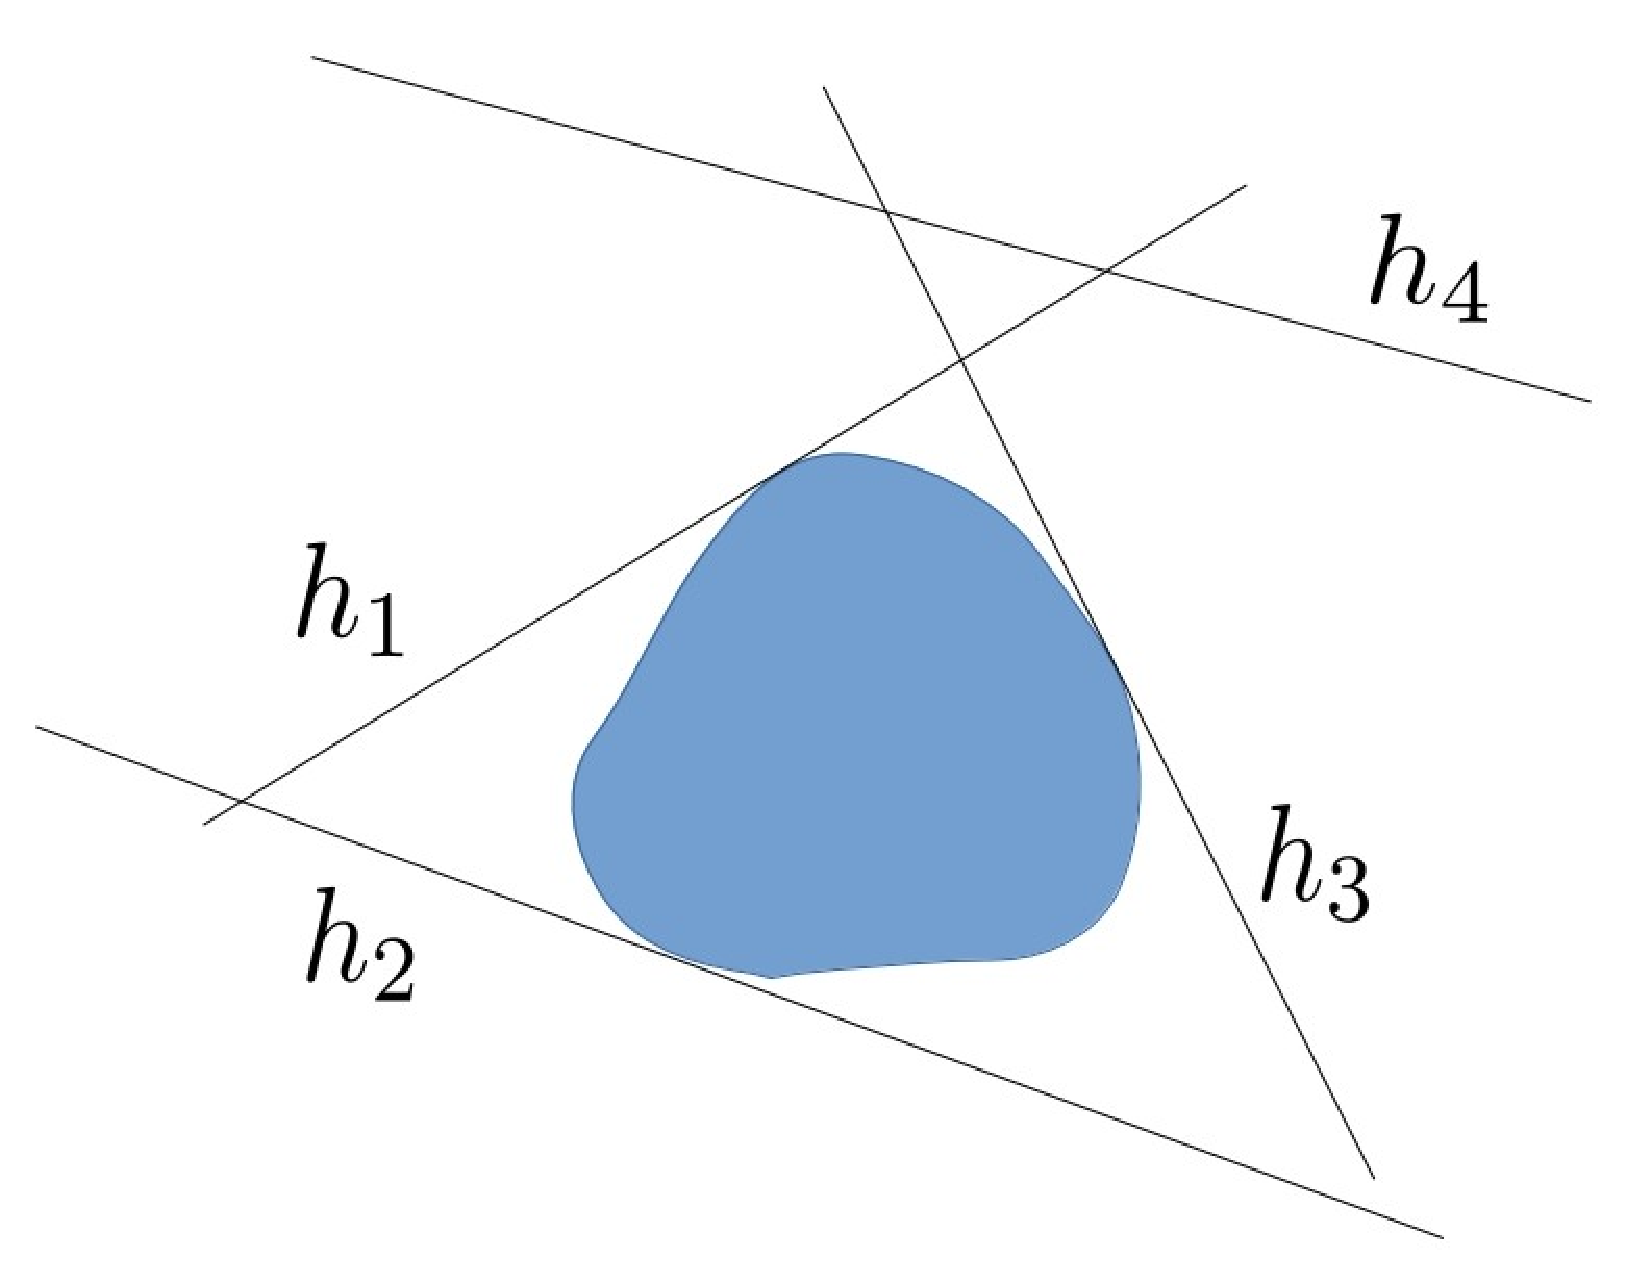
\includegraphics[scale=0.25]{images/Incosistency-example}
 \end{center}
 \caption{Пример несогласованных опорных чисел}
 \label{image:inconsistent}
\end{wrapfigure}

Оказывается, не всякий набор вещественных чисел является набором согласованных
опорных чисел (см. рис. \ref{image:inconsistent}).

Чтобы показать, насколько это важно, определим (следуя
\cite{Prince:1990:RCS:81024.81035}) так называемый \textit{основной объект} ---
тело, которое можно восстановить из опорных чисел, если о нем неизвестны никакие
другие априорные данные:

\begin{SmartDefinition}
 \label{def:basic-object}
 \textbf{Основным объектом} опорных чисел $h_{1}, h_{2}, \ldots, h_{m}$ по
 направлениям $u_{1}, u_{2}, \ldots, u_{m}$ называется многогранник $K^{0}$,
 определяемый как пересечение полупространств, ограниченных опорными плоскостями
 и содержащими начало координат $O$:
 \begin{equation}
  K^{0} = \bigcap \limits_{i = 1}^{m}\{(x, u_{i}) \leq h_{i}\}
 \end{equation}
\end{SmartDefinition}

В случае, если одно из опорных чисел было получено с большой погрешностью, может
оказаться, что заметная часть опорных чисел не будут учтена при построении
основного объекта. Так возникает вопрос \textit{построения оценки опорной
функции} --- такого набора согласованных опорных чисел
$h^{*} = (h^{*}_{1}, h^{*}_{2}, \ldots, h^{*}_{m})$, который был бы в некотором
смысле ближайшим к набору исходных чисел
$h^{0} = (h^{0}_{1}, h^{0}_{2}, \ldots, h^{0}_{m})$
, т. е. являлся бы решением следующей задачи
минимизации:

\begin{equation}
 \label{equation:abstract-problem}
 ||h - h^{0} ||_{X} \to \inf, \;\;\;\; s. t. \;\; h \in \mathfrak{C}
\end{equation}

где $X$ --- некоторая метрика в $\mathbb{R}^{n}$, а
$\mathfrak{C} \subset \mathbb{R}^{m}$ --- множество всех согласованных наборов
опорных чисел по направлениям $u_{1}, u_{2}, \ldots, u_{m}$.

\textbf{3. Исторический обзор.} Описанный выше подход для двумерного случая был
разработан в статьях Prince и Willsky \cite{Prince:1990:RCS:81024.81035},
изучавшими данные из компьютерной томографии,  и Lele, Kulkarni и Willsky
\cite{Lele:92}, изучавшими данные, полученные из лазерного радара. В них
доказывается так называемая \textbf{опорная теорема}:

\begin{SmartTheorem}
 \label{theorem:support-theorem}
  Набор опорных чисел $h = (h_{1}, h_{2}, \ldots, h_{m})$ по направлениям
  $u_{i} = (\cos \theta_{i}, \sin \theta_{i}) \in \mathbb{R}^{2},
  i = 1, \ldots, m$ является согласованным тогда и только тогда, когда

  \begin{equation}
   C h \geq 0
  \end{equation}

  где $C$ --- так называемая \textbf{опорная матрица}:
 \begin{equation}
  \left(
  \begin{array}{ccccccc}

   \scriptstyle     -sin(\theta_{2} - \theta_{M}) &
   \scriptstyle     sin(\theta_{1} - \theta_{M}) &
   \scriptstyle     0 &
   \scriptstyle     \ldots &
   \scriptstyle     0 &
   \scriptstyle     0 &
   \scriptstyle     sin(\theta_{2} - \theta_{1}) \\

   \scriptstyle      sin(\theta_{3} - \theta_{2}) &
   \scriptstyle      -sin(\theta_{3} - \theta_{1}) &
   \scriptstyle      sin(\theta_{2} - \theta_{1}) &
   \scriptstyle      \ldots &
   \scriptstyle      0 &
   \scriptstyle      0 &
   \scriptstyle      0 \\

   \scriptstyle      0 &
   \scriptstyle      sin(\theta_{4} - \theta_{3}) &
   \scriptstyle      -sin(\theta_{4} - \theta_{2}) &
   \scriptstyle      \ldots &
   \scriptstyle      0 &
   \scriptstyle      0 &
   \scriptstyle      0 \\

   \scriptstyle      \vdots &
   \scriptstyle      \vdots &
   \scriptstyle      \vdots &
   \scriptstyle      \ddots &
   \scriptstyle      \vdots &
   \scriptstyle      \vdots &
   \scriptstyle      \vdots \\

   \scriptstyle      0 &
   \scriptstyle      0 &
   \scriptstyle      0 &
   \scriptstyle      \ldots &
   \scriptstyle      -sin(\theta_{m - 1} - \theta_{m - 3}) &
   \scriptstyle      sin(\theta_{m - 2} - \theta_{m - 3}) &
   \scriptstyle      0 \\

   \scriptstyle      0 &
   \scriptstyle      0 &
   \scriptstyle      0 &
   \scriptstyle      \ldots &
   \scriptstyle      sin(\theta_{m} - \theta_{m - 1}) &
   \scriptstyle      -sin(\theta_{m} - \theta_{m - 2}) &
   \scriptstyle      sin(\theta_{m - 1} - \theta_{m - 2}) \\

   \scriptstyle      sin(\theta_{m} - \theta_{m - 1}) &
   \scriptstyle      0 &
   \scriptstyle      0 &
   \scriptstyle      \ldots &
   \scriptstyle      0 &
   \scriptstyle      sin(\theta_{1} - \theta_{m}) &
   \scriptstyle      -sin(\theta_{1} - \theta_{m - 1}) \\
  \end{array}
  \right)
 \end{equation}

\end{SmartTheorem}

Таким образом, множество всех согласованных наборов опорных чисел представляет
из себя конус, называемый \textit{опорным конусом}:

\begin{equation}
 \mathfrak{C} = \{h \in \mathbb{R}^{m} \; | \; C h \geq 0\}
\end{equation}

Следовательно, задача минимизации (\ref{equation:abstract-problem}) является
задачей квадратичного программирования в метрике $L_{2}$ и задачей линейного
программирования в метрике $L_{1}$:

\begin{equation}
 \label{equation:general-problem}
 ||h - h^{0} ||_{X} \to \inf, \;\;\;\; s. t. \;\; C h \geq 0
\end{equation}

Авторы приводят результаты решения этих задач минимизации, проводят анализ их
быстродействия, а также предлагают подходы, позволяющие учитывать априорные
знания о восстанавливаемых телах (такие как, например, кривизна).

Более сложным является рассмотрение задачи в трехмерном случае. Аналог теоремы
\ref{theorem:support-theorem} для трехмерного случая был доказан Karl, Kulkarni,
Verghese и Willsky \cite{Karl:1996:LTC:234032.234054}.

\begin{SmartTheorem}
 Набор опорных чисел $h = (h_{1}, h_{2}, \ldots, h_{m})$ по направлениям
 $u_{1}, u_{2}, \ldots, u_{m} \in \mathbb{R}^{3}$ является согласованным тогда и
 только тогда, когда неравенство

 \begin{equation}
 \label{equation:consistency-3d}
\left|\begin{array}{cc}
  h_{i} & u_{i}^{T} \\
  h_{j} & u_{j}^{T} \\
  h_{k} & u_{k}^{T} \\
  h_{l} & u_{l}^{T} \\
\end{array}\right|
  \left|\begin{array}{cc}
  1 & u_{i}^{T} \\
  1 & u_{j}^{T} \\
  1 & u_{k}^{T} \\
  1 & u_{l}^{T} \\
\end{array}\right|
\geq 0
\end{equation}

выполнено для всех четвёрок индексов $\{i, j, k, l\}$ таких, что сферический
треугольник, образованный векторами $u_{i}, u_{j}, u_{k}$ содержит в своей
внутренности вектор $u_{l}$ и не содержит никаких других опорных направлений из
$u_{1}, \ldots, u_{m}$ (такие четвёрки называются локальными положительными
конусами).
\end{SmartTheorem}

Таким образом, в трехмерном случае множество $\mathfrak{C}$ всех согласованных
опорных числе представляет из себя опорный конус, задаваемый уравнением
$C h \geq 0$, в котором строки опорной матрицы $C$ составлены из коэффициентов
уравнения (\ref{equation:consistency-3d}).

Авторы не доказали в статье оценок о количестве условий вида
(\ref{equation:consistency-3d}), однако произвели численный эксперимент по
построению условий для случайно выбранных опорных направлений. Из его
результатов можно предположить, что для случайно выбранных направлений число
уравнений растет примерно как $O(m^{2})$ (возможно, с логарифмическим
множителем).

Данный алгоритм был реализован Gregor и Rannou для данных из \\
магнитно-резонансной визуализации в статьях \cite{IMA:IMA10007} и
\cite{doi:10.1117/12.431168}. При этом авторы столкнулись с тем, что при больших
размерностях (порядка 100000 опорных направлений) время поиска локальных
положительных четвёрок было на порядок больше, чем время решения самой задачи
квадратичного программирования.

В связи с этим Gardner и Kiderlen \cite{4586384} решили переформулировать
исходную задачу в терминах точек касания:

\begin{equation}
\label{equation:gardner-kiderlen}
 ||\{(x_{i}, u_{i})\}_{i = 1}^{m} - h^{0}|| \to \inf \;\;\; s. t. \;\;
 (x_{i}, u_{i}) \geq (x_{j}, u_{i}), 1 \leq i \neq j \leq m
\end{equation}

где $x_{i} \in \mathbb{R}^{3}$ --- точки касания тела с опорной плоскостью,
имеющей нормаль $u_{i}$. Как нетрудно видеть, если решить задачу оптимизации
(\ref{equation:gardner-kiderlen}), то по полученным точкам касания $x^{*}_{i}$
можно получить согласованные опорные числа $h^{*}_{i} = (x^{*}_{i}, u_{i})$, а
по ним --- восстановить основной объект.

Преимущество данного подхода состоит в том, что условия согласованности
выписываются автоматически, и для их нахождения не требуется искать все
локальные положительные конусы. Тем не менее, основная проблема данного подхода,
а именно квадратичное число условий, сохраняется в данной постановке задачи.
Данная проблема делает описанный выше подход неприменимым к задачам большой
размерности.

В статьях Gardner, Kiderlen и Milanfar \cite{Gardner06convergenceof} и
Guntuboyina \cite{Guntuboyina2012} были сделаны исследования асимптотической
скорости сходимости методов оценки опорной функции, но были ли попытки сократить
число условий в описанных выше задачах, нам не известно.

\textbf{4. Расширение преобразования двойственности.}
Для того, чтобы обосновать предлагаемый нами подход, потребуется понятие
\textit{преобразования двойственности}. В соответствии с
\cite{Preparata:1985:CGI:4333}, определим его следующим образом:

\begin{SmartDefinition}
 Преобразованием двойственности называется преобразование $\delta$, переводящее
 точки в $\mathbb{R}^{3} \setminus \{O\}$ в плоскости:

 \begin{equation}
  \delta: (a, b, c) \mapsto \{a x + b y + c z = 1\},
 \end{equation}

 а плоскости, не содержащие начала координат $O$, -- в точки:

 \begin{equation}
  \delta: \{a x + b y + c z = 1\} \mapsto (a, b, c),
 \end{equation}
\end{SmartDefinition}

Преобразование двойственности также доопределяют на выпуклых многогранниках,
содержащих начало координат $O$ в своей внутренности:

\begin{SmartDefinition}
 Пусть $P$ --- выпуклый многогранник, содержащий начало координат $O$ в своей
 внутренности. Тогда двойственным многогранником $\delta(P)$ называется
 многогранник, имеющий вершины, двойственные плоскостям граней исходного
 многогранника, и грани, плоскости которых двойственны вершинам исходного
 многогранника.
\end{SmartDefinition}

В вычислительной геометрии часто используются следующие свойства преобразования
двойственности $\delta$ (см., например, \cite{Chazelle:1992:OAI:141741.141749}):

\begin{SmartTheorem}
\label{theorem:automorhism}
 $\delta$ сохраняет выпуклость для многогранников, содержащих начало координат:
 если $P$ -- выпуклый, $O \in Int(P)$, то $\delta(P)$ -- выпуклый,
 $O \in Int(\delta(P))$
\end{SmartTheorem}

\begin{SmartTheorem}
\label{theorem:self-inverse}
 $\delta$ обратно самому себе: если $P$ -- выпуклый, $O \in Int(P)$, то
 $\delta(\delta(P)) = P$
\end{SmartTheorem}

\begin{SmartTheorem}
\label{theorem:incidence-saving}
 $\delta$ сохраняет инцидентность: если $P$ -- выпуклый, $O \in Int(P)$, то
 грань $f$ и вершина $v$ многогранника $P$ инцидентны тогда и только тогда,
 когда инцидентны двойственные им вершина $\delta(f)$ и грань $\delta(v)$
 многогранника $\delta(P)$.
\end{SmartTheorem}

\begin{SmartTheorem}
\label{theorem:intersection-saving}
 $\delta$ сохраняет пересечение многогранников: если $P, Q$ -- выпуклые,
 $O \in Int(P)$, $O \in Int(Q)$, то
 $P \cap Q \neq \varnothing \Leftrightarrow
 \delta(P) \cap \delta(Q) \neq \varnothing$
\end{SmartTheorem}

Однако в данной работе нам потребуется доопределить преобразование
двойственности также и на двух более широких классах многогранников.

\begin{SmartDefinition}
 Пусть $K$ --- выпуклый многогранник, $O \in Int K$, а $p$ --- точка, лежащая в
 его внешности. Многогранником видимости для $K$ и $p$ будем называть
 объединение отрезков $[p, q]$ таких, что точка $q \in \partial K$ видна из
 точки $p$:
 \begin{equation}
  P(K, p) = \bigcup \limits_{q \in \partial K, [p, q] \cap Int K = \varnothing}
  [p, q]
 \end{equation}
Многогранник $P$ называется \textbf{многогранником видимости}, если \
$P = P(K, p)$ для некоторого многогранника $K$ и точки $p$.
\end{SmartDefinition}

\begin{SmartDefinition}
 \textbf{Многогранником двойственной видимости} называется выпуклый
 многогранник $P$, являющийся пересечением такого набора полупространств
 \begin{equation}
 \label{equation:halfspace}
  \{a_{i} x + b_{i} y + c_{i} z + d_{i} \leq 0 \}, \;\;\; i = 1, \ldots, s,
 \end{equation}
 что ровно одно из них не содержит начало координат $O$ в своей внутренности, а
 остальные --- содержат $O$ в своей внутренности, т. е. $d_{1} > 0$ и
 $d_{i} < 0, i = 2, \ldots, s$
\end{SmartDefinition}

Очевидно, что такой класс многогранников является самым простым способом
расширить исходную область определения $\delta$: каждый выпуклый многогранник
$P$ такой, что $O \in Int(P)$ можно представить в виде пересечения
полупространств такого же вида, только при условии, что у всех них свободные
коэффициенты отрицательны:

\begin{equation}
 P = \{a_{i} x + b_{i} y + c_{i} z + d_{i} \leq 0 \}, \;\;\;
 d_{i} < 0, \;\;\;
 i = 1, \ldots, s
\end{equation}

Теперь доопределим преобразование двойственности $\delta$ на введённых классах
многогранников. Для этого докажем следующую теорему:

\begin{SmartTheorem}
\label{theorem:duality-expansion}
 Пусть $P$ --- многогранник видимости, причем $P = P(K, p)$. Пусть
 $p, q_{1}, q_{2}, \ldots, q_{s}$ --- вершины $P$, $f_{1}, \ldots, f_{r}$ ---
 плоскости граней $P$. Обозначим их двойственные образы следующим образом:
 \begin{equation}
  \delta(p) = \{a_{p} x + b_{p} y + c_{p} z = 1\}
 \end{equation}
 \begin{equation}
  \delta(q_{i}) = \{a_{i} x + b_{i} y + c_{i} z = 1\}
 \end{equation}
 \begin{equation}
  \delta(f_{i}) = g_{i}
 \end{equation}
 Обозначим многогранник $D = Hull(g_{1}, \ldots, g_{r})$. Тогда верны следующие
 утверждения:
 \begin{enumerate}
  \item Точки $g_{1}, \ldots, g_{r}$ находятся в экстремальном положении, то
  есть лежат на границе своей выпуклой оболочки: $g_{i} \in \partial D$
  \item $D$ есть многогранник двойственной видимости, представимый следующим
  образом:
  \begin{equation}
  \label{equation:dual-visibility-polyhedron}
   D = \{-a_{p} x - b_{p} y - c_{p} z + 1 \leq 0\} \cap
   \bigcap \limits_{i = 1}^{s} \{a_{i} x + b_{i} y + c_{i} z - 1 \leq 0\}
  \end{equation}
 \end{enumerate}
\end{SmartTheorem}

\textbf{Доказательство.}

Рассмотрим следующие многогранники:

\begin{equation}
 D_{1} = \bigcap \limits_{i = 1}^{s} \{a_{i} x + b_{i} y + c_{i} z - 1 \leq 0\}
\end{equation}
\begin{equation}
 D_{2} = D_{1} \cap \{a_{p} x + b_{p} y + c_{p} z - 1 \leq 0\}
\end{equation}
\begin{equation}
 D' = D_{1} \cap \{-a_{p} x - b_{p} y - c_{p} z + 1 \leq 0\}
\end{equation}
По определению $D_{1}$ и $D_{2}$ являются выпуклыми и содержат начало координат
в своей внутренности. Нетрудно видеть, что

\begin{equation}
 \delta(D_{1}) = K, \;\; \delta(D_{2}) = Hull(K, p),
\end{equation}

поскольку преобразование двойственности сохраняет отношение инцидентности.
Также из определения этих многогранников следует, что
\begin{equation}
 D_{1} = D' \cup D_{2}, \;\;
 \partial D_{1} \cup \delta(p) = \partial D' \cup \partial D_{2}
\end{equation}

Фиксируем некоторую плоскость $f_{i}$ грани многогранника $P$. Возможны два
случая:

\begin{enumerate}
 \item Грань $P$, лежащая в $f_{i}$, есть грань многогранника $K$. Тогда $g_{i}$
 есть вершина многогранника $D_{1}$, не лежащая на границе $D_{2}$.
 Следовательно, $g_{i} \in \partial D'$.
 \item Грань $P$, лежащая в $f_{i}$, есть грань многогранника $Hull(K, p)$, не
 являющаяся гранью $K$. Тогда она инцидента вершине $p$ и, следовательно,
 $g_{i} \in \delta(p) \subset \partial D'$.
\end{enumerate}

Таким образом, все $g_{i} \in \partial D'$, а поскольку $D'$ по определению
выпуклый, то $g_{i}$ находятся в экстремальном положении, и их выпуклая оболочка
$D = Hull(g_{1}, \ldots, g_{r}) \subset D'$. Обратное включение $D' \subset D$
также легко доказать: если $g$ --- вершина $D'$, то либо $g$ -- вершина $D_{1}$,
либо $g \in \delta(p)$. В обоих случаях $g = g_{i}$ для некоторого $i$.

$\square$

Данная теорема позволяет естественным образом доопределить преобразование
двойственности на двух введённых выше классах многогранников.

\begin{SmartDefinition}
 Пусть $P$ --- многогранник видимости, тогда положим $\delta(P) = D$, где $D$
 --- многогранник, определяемый соотношением
 (\ref{equation:dual-visibility-polyhedron}).
\end{SmartDefinition}
\begin{SmartDefinition}
 Пусть $D$ --- многогранник двойственной видимости, тогда его нетрудно
 представить в виде (\ref{equation:dual-visibility-polyhedron}). Положим
 $\delta(D) = P$ из теоремы \ref{theorem:duality-expansion}.
\end{SmartDefinition}

Смысл этого доопределения состоит в том, чтобы доказать аналоги теорем
\ref{theorem:automorhism}, \ref{theorem:self-inverse},
\ref{theorem:incidence-saving}, \ref{theorem:intersection-saving} для
расширенного преобразования. Аналоги первых двух из этих теорем вложены в
определения, аналог теоремы \ref{theorem:incidence-saving} также тривиален.

Аналог теоремы \ref{theorem:intersection-saving} можно сформулировать в
следующем виде:

\begin{SmartTheorem}
 Многогранники двойственной видимости $P$ и $Q$ пересекаются тогда и только
 тогда, когда пересекаются двойственные им многогранники видимости
 $\delta(P)$ и $\delta(Q)$.
\end{SmartTheorem}

Из этой теоремы вытекает тривиальное следствие:

\begin{SmartLemma}
\label{lemma:expanded-intersection-saving}
 Пусть $K$ --- выпуклый многогранник, $O \in Int K$. Тогда многогранники
 $K_{1} = K \cap \{a_1 x + b_1 y + c_1 z + 1 \leq 0\}$,
 $K_{2} = K \cap \{a_2 x + b_2 y + c_2 z + 1 \leq 0\}$.
 являются многогранниками двойственной видимости. Обозначим
 $p_1 = \delta(\{a_1 x + b_1 y + c_1 z + 1 = 0\})$,
 $p_2 = \delta(\{a_2 x + b_2 y + c_2 z + 1 = 0\})$.
 Тогда многогранники $K_{1}$ и $K_{2}$ пересекаются тогда и только тогда, когда
 пересекаются двойственные им многогранники видимости $P(p_1, \delta(K))$ и
 $P(p_2, \delta(K))$, или, что то же самое,
 \begin{equation}
  K_{1} \cap K_{2} \neq \varnothing \Leftrightarrow
  [p_1, p_2] \cap \delta(K) = \varnothing
 \end{equation}
\end{SmartLemma}

Пересечение двух многогранников видимости $P(p_1, \delta(K))$ и
$P(p_2, \delta(K))$ , соответствующих одному многограннику $\delta(K)$,
очевидно, можно интерпретировать как факт, что точки $p_1$ и $p_2$ "видят" друг
друга, то есть многогранник $\delta(K)$ "не закрывает" одну точку от другой.

\textbf{5. Метод исключения избыточных условий.} Рассмотрим задачу в терминах
точек касания в метрике $L_{\infty}$. Если ввести дополнительную переменную
$\varepsilon$, то задачу можно переписать в следующем виде:

\begin{equation}
\label{equation:infinity-problem}
 \varepsilon \to \inf \;\;\;
 s. t. \;\; (x_{i}, u_{i}) \geq (x_{i}, u_{j}), \;\;\;
 |(x_{i}, u_{i}) - h_{i}| \leq \varepsilon
\end{equation}

Оказывается, при такой постановке задачи большая часть условий вида
$(x_{i}, u_{i}) \geq (x_{i}, u_{j})$ являются избыточными.
В основе предлагаемого метода лежит \textit{достаточное условие избыточности}.

Мы будем рассматривать его вне контекста задачи оптимизации
(\ref{equation:infinity-problem}), поскольку в дальнейшем метод понадобится и
для задач в метриках $L_{1}$ и $L_{2}$.

Итак, рассмотрим систему ограничений:

\begin{equation}
\label{equation:all-constraints}
 (x_{i}, u_{i}) \geq (x_{i}, u_{j}), \;\;\;
 |(x_{i}, u_{i}) - h_{i}| \leq \varepsilon
\end{equation}

\begin{SmartTheorem}\label{theorem:exhaustive-conditions}
Пусть система ограничений (\ref{equation:all-constraints}) разрешима
для некоторого $\varepsilon^{0}$. Обозначим многогранник

\begin{equation}
\label{equation:upper-bounds-polyhedron}
 K = \bigcap \limits_{i = 1}^{m}\{(x, u_{i}) \leq h_{i} + \varepsilon^{0}\}
\end{equation}

Пусть $\delta$ - полярное преобразование двойственности.
Тогда если отрезок, соединяющий точки
$\delta(\{(x, u_{i}) = h_{i} - \varepsilon^{0}\})$ и
$\delta(\{(x, u_{j}) = h_{j} - \varepsilon^{0}\})$ пересекает
$\delta(K)$, то условия $(x_{i}, u_{i}) \geq (x_{j}, u_{i})$ и
$(x_{j}, u_{j}) \geq (x_{i}, u_{j})$ избыточны в системе ограничений
(\ref{equation:all-constraints}).
\end{SmartTheorem}

\textbf{Доказательство.}
Пусть система ограничений (\ref{equation:all-constraints}) разрешима
для некоторого $\varepsilon^{0}$. Тогда, как всякая задача линейного
программирования, она имеет оптимальное решение
$x = x^{*}, \varepsilon = \varepsilon^{*}$, удовлетворяющее следующим условиям:

\begin{equation}
 (x_{i}, u_{i}) \geq (x_{i}, u_{j}), \;\;\;
 |(x_{i}, u_{i}) - h_{i}| \leq \varepsilon^{0}
\end{equation}

Из ограничения  $|(x_{i}, u_{i}) - h_{i}| \leq \varepsilon^{0}$ можно
получить два условия: ограничение на $(x_{i}, u_{i})$ сверху:

\begin{equation}
 (x_{i}, u_{i}) \leq h_{i} + \varepsilon^{0}
\end{equation}

и снизу:

\begin{equation}
\label{equation:lower-bound}
 (x_{i}, u_{i}) \geq h_{i} - \varepsilon^{0}
\end{equation}

Ограничение $(x_{i}, u_{i}) \geq (x_{i}, u_{j})$ означает, что точка $x_{i}$
реализует максимум величины проекции на направление $u_{i}$ среди всех точек
касания. Следовательно, для всех точек касания $x = x_{k}$ выполнено условие:

\begin{equation}
 (x, u_{i}) \leq h_{i} + \varepsilon^{0}
\end{equation}

Повторяя это утверждение для всех $i = 1, 2, \ldots, m$, получим, что все точки
касания лежат в многограннике $K$, введённом в формулировке теоремы
(\ref{equation:upper-bounds-polyhedron}). Отсюда и из
(\ref{equation:lower-bound}) следует, что каждая точка касания $x_{i}$ лежит
в многограннике $K_{i}$, определяемом следующим образом:

\begin{equation}
 K_{i} = K \cap \{(x_{i}, u_{i}) \geq h^{0}_{i} - \varepsilon^{0}\}
\end{equation}

Докажем, что если многогранники $K_{i}$ и $K_{j}$ не пересекаются, то условия
$(x_{i}, u_{i}) \geq (x_{j}, u_{i})$ и $(x_{j}, u_{j}) \geq (x_{i}, u_{j})$
избыточны в системе ограничений (\ref{equation:all-constraints}).

Действительно, из $K_{i} \cap K_{j} = \varnothing$ следует, что плоскость
$\{(x_{i}, u_{i}) = h_{i} - \varepsilon^{0}\}$ не пересекает многогранник
$K_{j}$, а плоскость $\{(x_{j}, u_{j}) = h_{j} - \varepsilon^{0}\}$ не
пересекает многогранник $K_{i}$.

Тогда из условий $x_{i} \in K_{i}$ и $x_{j} \in K_{j}$ следует, что
$(x_{i}, u_{j}) < h - \varepsilon^{0}$ и
$(x_{j}, u_{j}) \geq h - \varepsilon^{0}$, откуда имеем условие
$(x_{i}, u_{j}) \leq (x_{j}, u_{j})$. Аналогично из условий $x_{i} \in K_{i}$ и
$x_{j} \in K_{j}$ можно вывести $(x_{j}, u_{i}) \leq (x_{i}, u_{i})$.

Для завершения доказательства теоремы остаётся доказать, что многогранники
$K_{i}$ и $K_{j}$ не пересекаются тогда и только тогда, когда отрезок,
соединяющий точки $\delta(\{(x, u_{i}) = h^{0}_{i} - \varepsilon^{0}\})$ и
$\delta(\{(x, u_{j}) = h_{j} - \varepsilon^{0}\})$ пересекает $\delta(K)$.
Но это утверждение является прямым следствием леммы
(\ref{lemma:expanded-intersection-saving}).

$\square$

В метрике $L_{1}$ задачу (\ref{equation:gardner-kiderlen}) можно записать в
следующем виде:

\begin{equation}
\label{equation:initial-l1-problem}
\begin{split}
 I = \sum \limits_{i = 1}^{m} |(x_{i}, u_{i}) - h_{i}| \to \inf \\
 s. t. (x_{i}, u_{i}) \geq (x_{j}, u_{i}), 1 \leq i \neq j \leq m,
\end{split}
\end{equation}

а в метрике $L_{2}$ -- в следующем:

\begin{equation}
\label{equation:initial-l2-problem}
\begin{split}
 I = \sum \limits_{i = 1}^{m} ((x_{i}, u_{i}) - h_{i})^{2} \to \inf \\
 s. t. (x_{i}, u_{i}) \geq (x_{j}, u_{i}), 1 \leq i \neq j \leq m
\end{split}
\end{equation}

Между тем, довольно естественно ожидать что полученные оптимальные точки касания
будут удовлетворять условию
$|(x^{*}_{i}, u_{i}) - h_{i}| \leq \varepsilon^{0}$
для некоторого фиксированного $\varepsilon^{0} > 0$ при соображении малости
погрешности. Если наложить на задачи (\ref{equation:initial-l1-problem}) и
(\ref{equation:initial-l2-problem}) дополнительные ограничения

\begin{equation}
\label{equation:additional-constraints}
 |(x_{i}, u_{i}) - h_{i}| \leq \varepsilon^{0},
\end{equation}

то задачу (\ref{equation:initial-l1-problem}) можно будет переформулировать в
следующем виде:

\begin{equation}
\label{equation:reduced-l1-problem}
\begin{split}
 I = \varepsilon_{1} + \ldots + \varepsilon_{m} \to \inf \\
 s. t. (x_{i}, u_{i}) \geq (x_{j}, u_{i}), 1 \leq i \neq j \leq m, \\
 | (x_{i}, u_{i}) - h_{i} | \leq \varepsilon_{i}, i = 1, \ldots, m, \\
 0 \leq \varepsilon_{i} \leq \varepsilon^{0}, i = 1, \ldots, m,
\end{split}
\end{equation}

а задачу (\ref{equation:initial-l2-problem}) -- в следующем:

\begin{equation}
\label{equation:reduced-l1-problem}
\begin{split}
 I = \varepsilon_{1}^{2} + \ldots + \varepsilon_{m}^{2} \to \inf \\
 s. t. (x_{i}, u_{i}) \geq (x_{j}, u_{i}), 1 \leq i \neq j \leq m, \\
 | (x_{i}, u_{i}) - h_{i} | \leq \varepsilon_{i}, i = 1, \ldots, m, \\
 0 \leq \varepsilon_{i} \leq \varepsilon^{0}, i = 1, \ldots, m,
\end{split}
\end{equation}

Строго говоря, такие две задачи не являются эквивалентными исходным. Однако,
из соображений локальности, мы считаем, что решения последних двух задач будут
в некотором смысле близки к решениям первых.

Итак, приведём алгоритм простроения системы неизбыточных ограничений:

\begin{enumerate}
 \item $S = \varnothing$
 \item По исходным опорным данным $u_{i}, h_{i}, i = 1, \ldots, m$
 построить тело $K^{0}$ как пересечение полупространств:
 \begin{equation}
 \label{equation:naive-body}
  K^{0} = \bigcap \limits_{i = 1}^{m} \{(u_{i}, x) \leq h_{i}\}
 \end{equation}
 \item Пусть $A_{1}, \ldots A_{s}$ --- вершины тела $K^{0}$. Вычислить опорные
 числа тела $K^{0}$ по направлениям $u_{i}, i = 1, \ldots, m$ следующим образом:
 \begin{equation}
  h^{0}_{i} = \max \limits_{j = 1, \ldots, s} (u_{i}, A_{j})
 \end{equation}
 \item Вычислить $L_{\infty}$-расстояние от полученных опорных чисел до
 исходных:
 \begin{equation}
  \varepsilon^{0} = \max \limits_{i = 1, \ldots, m} |h_{i} - h^{0}_{i}|
 \end{equation}
 \item Построить многогранник $D_{\varepsilon^{0}}$ как выпуклую оболочку
 двойственных образов верхних плоскостей:
 \begin{equation}
  D_{\varepsilon^{0}} =
  Hull \left\{
  \delta(\{(x, u_{i}) = h_{i} + \varepsilon^{0}\})
  \right\}_{i = 1}^{m}
 \end{equation}
 \item Построить двойственные образы нижних плоскостей:
 \begin{equation}
  p_{i} = \delta(\{(x, u_{i}) = h_{i} - \varepsilon^{0}\})
 \end{equation}
 \item Для всех $i, j = 1, \ldots, m, i \neq j$ проверить следующее условие:
 \begin{equation}
  [p_{i}, p_{j}] \cap D_{\varepsilon^{0}} = \varnothing
 \end{equation}
 Если оно выполняется, то добавить неравенства
 \begin{equation}
 \begin{split}
  (u_{i}, x_{i}) \geq (u_{i}, x_{j}) \\
  (u_{j}, x_{j}) \geq (u_{j}, x_{i})
 \end{split}
 \end{equation}
 в систему ограничений $S$.
\end{enumerate}

Вообще говоря, программист на свой страх и риск может в шаге 4 приведенного
алгоритма уменьшить полученнное отклонение на некоторый множитель, для того
чтобы как можно сильнее сократить число ограничений:

\begin{equation}
 \varepsilon' = f \varepsilon^{0}, \;\; 0 < f < 1,
\end{equation}

однако, в отличие от $\varepsilon^{0}$, для $\varepsilon'$ нельзя
гарантировать согласованность системы ограничений
(\ref{equation:all-constraints}). При этом может оказаться, что
$\varepsilon' < \varepsilon^{*}$, и тогда система
(\ref{equation:all-constraints}) будет несогласованна. Полученное при
прохождении остальных шагов алгоритма задача не будет эквивалентна
исходной, и её решение не будет удовлетворять всем условиям согласованности.

\textbf{6. Реализация алгоритма.} В качестве входных данных для программы
использовались теневые контуры, полученные в результате фотографирования
драгоценных камней. Теневые контуры представляли из себя проекции вдоль
некоторых горизонтальных направлений $\nu_{i}, i = 1, \ldots, n$. Каждый такой
контур можно является многоугольником на плоскости $(\nu_{i}, x) = 0$.
Рассматривавшиеся производственные теневые контуры могли быть незамкнутыми,
поскольку сторона контура, соответствующая грани, на которой стоял камень на
подставке во время фотографирования, часто не включалась в описание контура.
Описание каждого контура представляло из себя список пар координат концов сторон
контура.

Для упрощения задачи над теневыми контурами производилась следующая
предобработка:

\begin{enumerate}
 \item Если контур являлся незамкнутым, то он замыкался: между соседними
 сторонами добавлялась дополнительная сторона
 \item Вычислялся центр масс $C$ объединения всех контуров, и из всех координат
 концов сторон вычитался вектор $OC$. Это делалось для того, чтобы гарантировать
 положительность всех опорных чисел (Опорные числа положительны если и только
 если тело содержит начало координат $O$ в своей внутренности).
 \item Невыпуклые контуры заменялись своей выпуклой оболочкой.
\end{enumerate}

Очевидно, что процесс получения теневого контура можно интерпретировать как
измерение опорной функции тела на большом круге сферы, т. е. каждый теневой
контур по сути представляет из себя непрерывное семейство измерений опорной
функции тела. Поскольку такие измерения получаются экспериментальным путем, то
для нескольких контуров может не найтись выпуклого многогранника, им
соответствующего.

Чтобы согласовать контуры между собой, из них извлекались нормали всех сторон
всех контуров $u_{i}, i = 1, \ldots, n$ и расстояния от начала координат до
сторон $h_{i}$. Эти данные интерпретировались как измерения опорной функции
исходного тела по опорным направлениям $u_{i}$. Очевидно, что согласованность
опорных чисел $h_{i}$ является необходимым условием согласованности теневых
контуров. Целью работы программы является построение таких согласованных чисел
$h^{*}_{i}$, которые бы были наиболее близки к исходным.

Алгоритм построения системы неизбыточных ограничений был реализован на
основе API библиотеки алгоритмов вычислительной геометрии CGAL \cite{cgal}. В 
качестве алгоритма построения выпуклой оболочки был использован стандартный
алгоритм Quickhull \cite{Barber:1996:QAC:235815.235821} из пакета трехмерных
выпуклых оболочек \cite{cgal:hs-ch3-15a}.

Для нахождения пересечения
полупространств в уравнении (\ref{equation:naive-body}) все плоскости, задающие
полупространства, сначала отображались в двойственные им точки с помощью 
преобразования двойственности $\delta$, затем строилась выпуклая оболочка
полученных точек, вычислялись уравнения плоскостей граней полученного
двойственного многогранника $\delta(K^{0})$, и на их основе
вычислялись координаты вершин многогранника $K^{0}$ из уравнения
(\ref{equation:naive-body}).

Для быстрой проверки пересечения
отрезка и многогранника использовалась структура данных AABB-дерево
\cite{cgal:atw-aabb-15a}, позволяющая автоматически распараллеливать запросы
на проверки пересечения.

С помощью алгоритма построения системы неизбыточных ограничений строилась
система ограничений задачи, к которым затем добавлялись условия локальности
$|(x_{i}, u_{i}) - h_{i}| < \varepsilon^{0}$ для $L_{\infty}$ задачи, либо
$|(x_{i}, u_{i}) - h_{i}| < \varepsilon_{i}$ для $L_{1}$ и $L_{2}$ задач.

Полученные задачи решались с помощью следующих пакетов для решения задач
оптимизации:

\begin{enumerate}
 \item GLPK \cite{glpk} использовался для решения $L_{\infty}$ и $L_{1}$ задач
 и для генерации задач в формате MPS, который затем подавался на вход другим
 решателям.
 \item CLP \cite{clp} использовался для решения $L_{\infty}$ и $L_{1}$ задач.
 \item Ipopt \cite{ipopt, DBLP:journals/mp/WachterB06}, решатель на основе
 метода внутренней точки, использовался для решения $L_{\infty}$, $L_{1}$ и
 $L_{2}$ задач с помощью С++ API для разделяемой библиотеки.
 \item IBM ILOG CPLEX \cite{cplex} использовался для решения
 $L_{\infty}$ и $L_{1}$ задач в формате MPS или LP.
\end{enumerate}

В методе внутренней точки, реализованном в решателе Ipopt, помимо описания
задачи оптимизации требуется указать начальную точку алгоритма. От того,
насколько данная точка близка к точке минимума, существенно зависит
быстродействие алгоритма. Поэтому в качестве начального положения точек касания
$x_{i}$ были взяты точки касания пересечения полупространств из уравнения
(\ref{equation:naive-body}):

\begin{equation}
 (u_{i}, x^{0}_{i}) = \max \limits_{j = 1, \ldots, N} (u_{i}, y_{j}),
\end{equation}

где $y_{j}, j = 1, \ldots, N$ --- коодинаты вершин многогранника $K^{0}$ из
уравнения (\ref{equation:naive-body}).

В результате работы решателей получался набор точек касания
$x^{*}_{i}, i = 1, \ldots, m$, на основе которых строился набор опорных чисел
$h^{*}_{i} = (x^{*}_{i}, u_{i})$. По этим числам и происходило восстановление
трехмерного тела как пересечения полупространств:

\begin{equation}
 K^{*} = \bigcap \limits_{i = 1}^{m} \{(x, u_{i}) \leq h^{*}_{i}\}
\end{equation}

Вычисление этого многогранника осуществлялось точно так же, как и вычисление
многогранника $K^{0}$ (см. выше).

\textbf{7. Результаты тестирования алгоритма.}
Реализованный алгоритм тестировался на ЭВМ с 4-ядерным процессором
Intel Core i5-2500 CPU с частотой 3.30 GHz, ОЗУ 16 ГБ и операционной
системой Ubuntu 14.04 LTS.

Данная статья не преследует цель сравнить скорость тех или иных решателей,
упомянутых выше, поскольку все они использовались со стандартными настройками
конфигурации и, возможно, для тех или иных пакетов был использован не самый
оптимальный выбор настроек. Тем не менее, чтобы дать читателю понятие о
скорости алгоритма, приведем здесь те результаты, которые удалось получить.

Получить решение линейных задач (т. е. $L_{1}$ и $L_{\infty}$) за приемлемое
время удалось с помощью пакетов IBM ILOG CPLEX и Ipopt. Единственным решателем,
который смог справиться с квадратичной задачей, оказался Ipopt. По этой причине
здесь будут приведены только результаты, полученные с помощью этих двух пакетов.

В документации Ipopt указано, что его производительность может меняться на
порядки в зависимости от того, какой пакет линейной алгебры к нему подключен.
Наиболее быструю производительность пакета Ipopt для данной задачи удалось
получить с использованием метода MA57 из пакета HSL \cite{hsl} и пакета
OpenBLAS \cite{xianyi2013openblas}, использованного в качестве реализации
библиотеки основных функций линейной алгебры (BLAS).

В качестве входных данных алгоритма были использован набор из 200 теневых
контуров, полученных в результате фотографирования реального камня. Каждый
контур содержал в среднем примерно по 15 сторон: общее число сторон во всех
контурах равнялось 2912. Для проверки асимптотики скорости работы алгоритма из
данного набора контуров равномерно выбирались поднаборы из
$10, 20 , 30, \ldots, 180, 190, 200$ контуров и подавались в качестве входных
данных для алгоритма.

\begin{figure}[hh]
 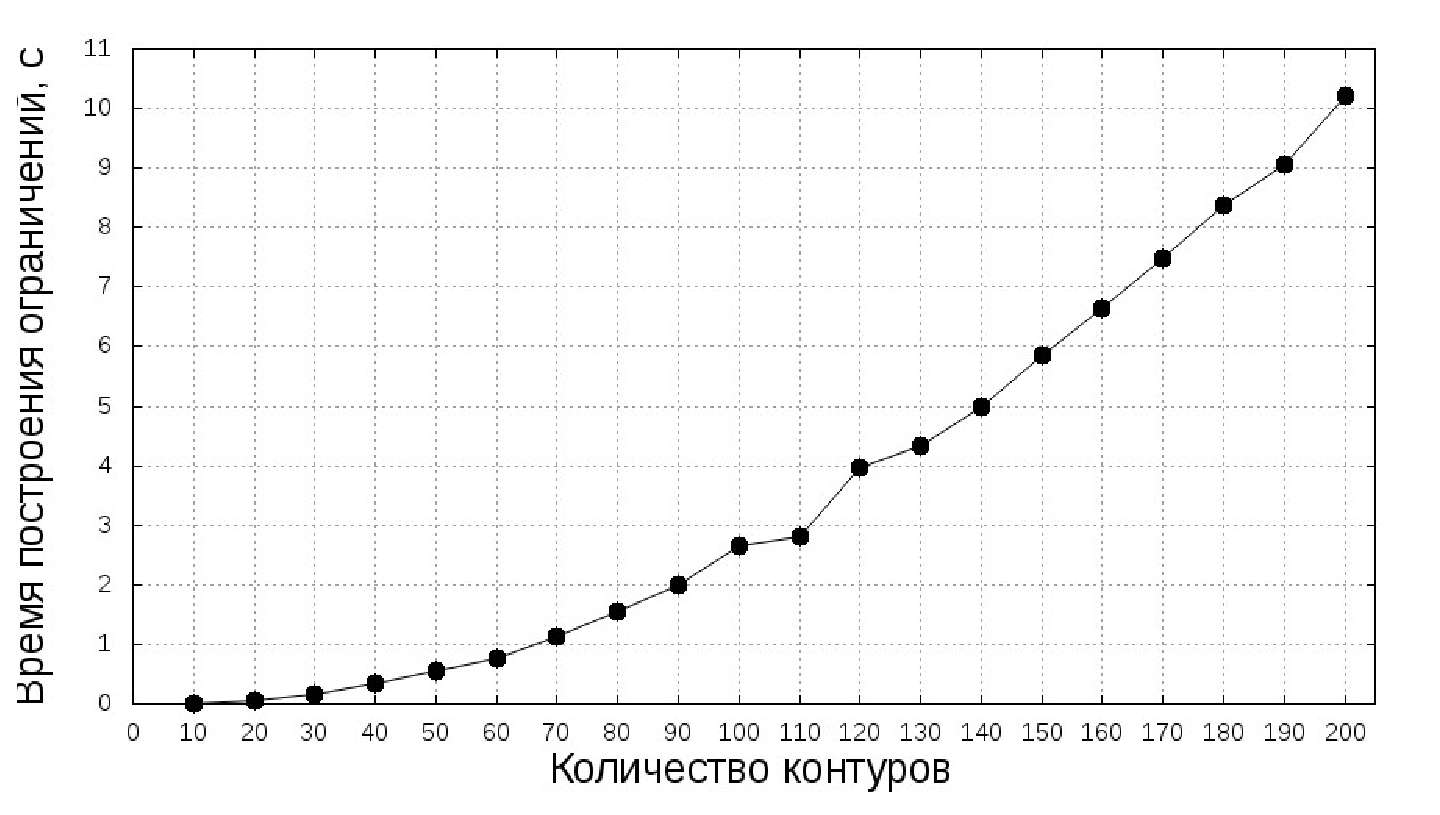
\includegraphics[width=\textwidth]{images/Problem-preparation-time-graph}
 \caption{Время работы алгоритма нахождения системы неизбыточных условий.}
 \label{Problem-preparation-time-graph}
\end{figure}

На рисунке \ref{Problem-preparation-time-graph} показан график времени работы
алгоритма построения системы неизбыточных условий. Очевидно, что данный алгоритм
осуществляет квадратичный перебор всех пар опорных направлений, и как видно по
графику, квадратичная сложность имеет место и на практике.

Какую пользу приносит предлагаемый алгоритм? Сколько условий он позволяет
отбросить? На рисунке \ref{Reduced-constraints-count-graph} показаны графики
числа ограничений до и после применения алгоритма, а на рисунке
\ref{Reduced-constraints-ratio-graph} -- график отношения этих величин. Таким
образом, в рассмотренном примере удалось сократить более 80\% ограничений.

\begin{figure}[hh]
 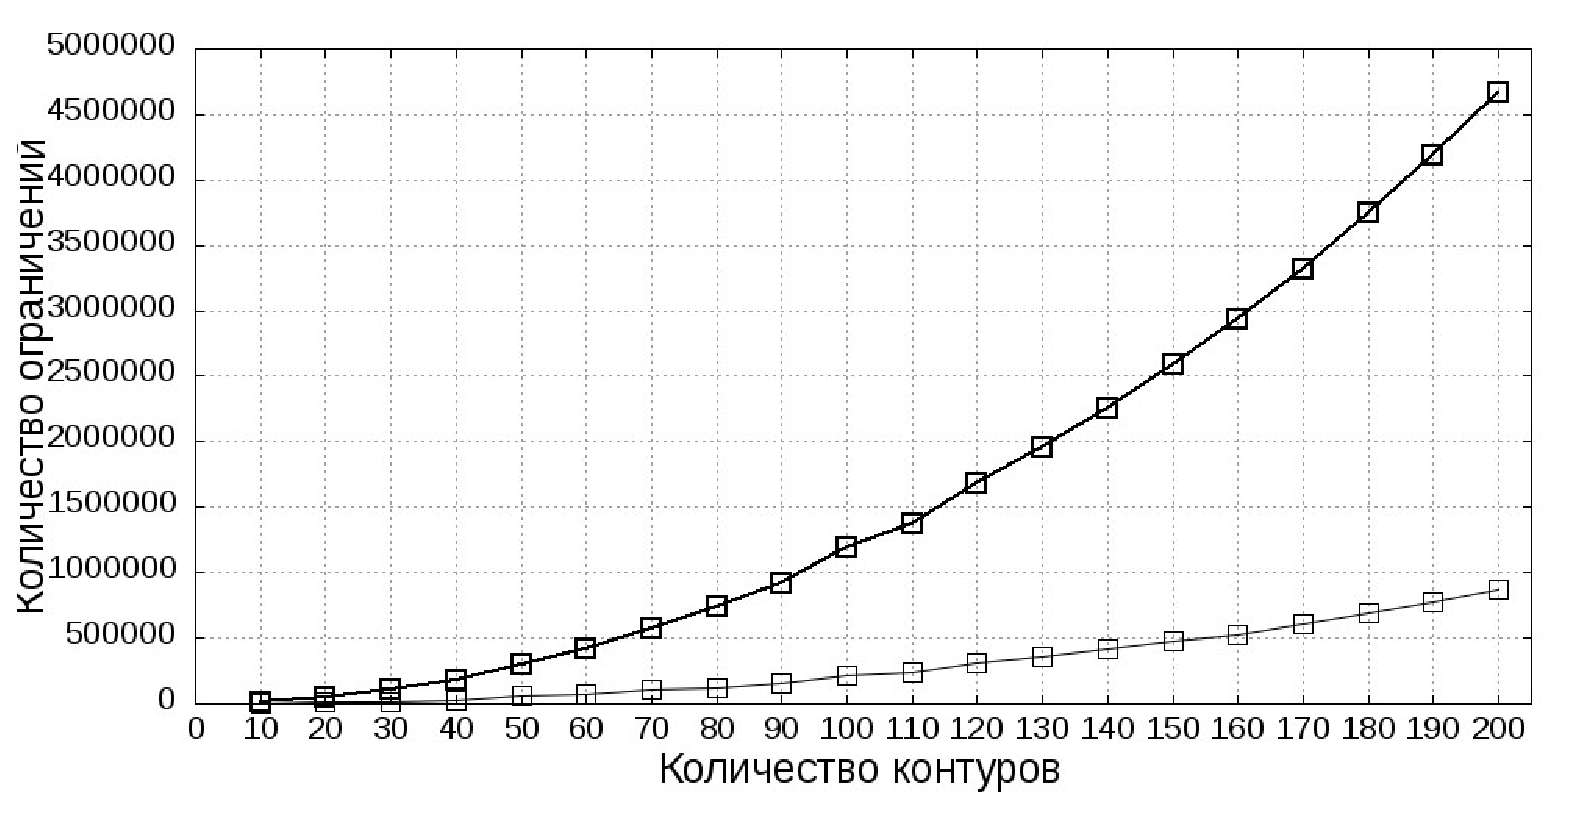
\includegraphics[width=\textwidth]{images/Reduced-constraints-count-graph}
 \caption{Количество ограничений. \textbf{Жирным цветом} помечен график общего
 числа ограничений, обычным цветом -- график числа неизбыточных ограничений.}
 \label{Reduced-constraints-count-graph}
\end{figure}

\begin{figure}[hh]
 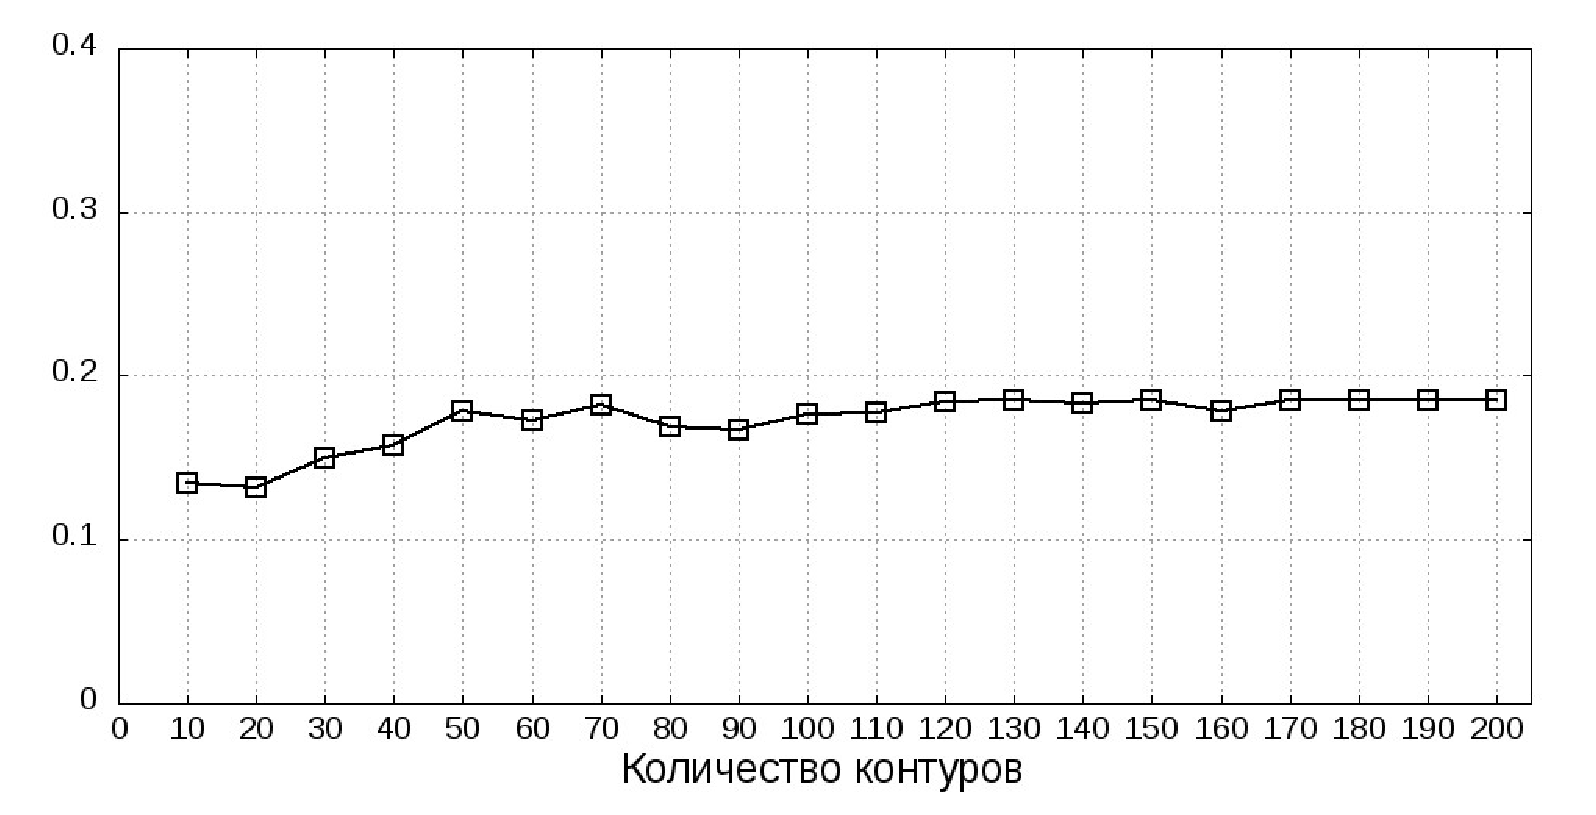
\includegraphics[width=\textwidth]{images/Reduced-constraints-ratio-graph}
 \caption{Отношение числа неизбыточных ограничений к общему числу ограничений}
 \label{Reduced-constraints-ratio-graph}
\end{figure}

\begin{figure}[p]
 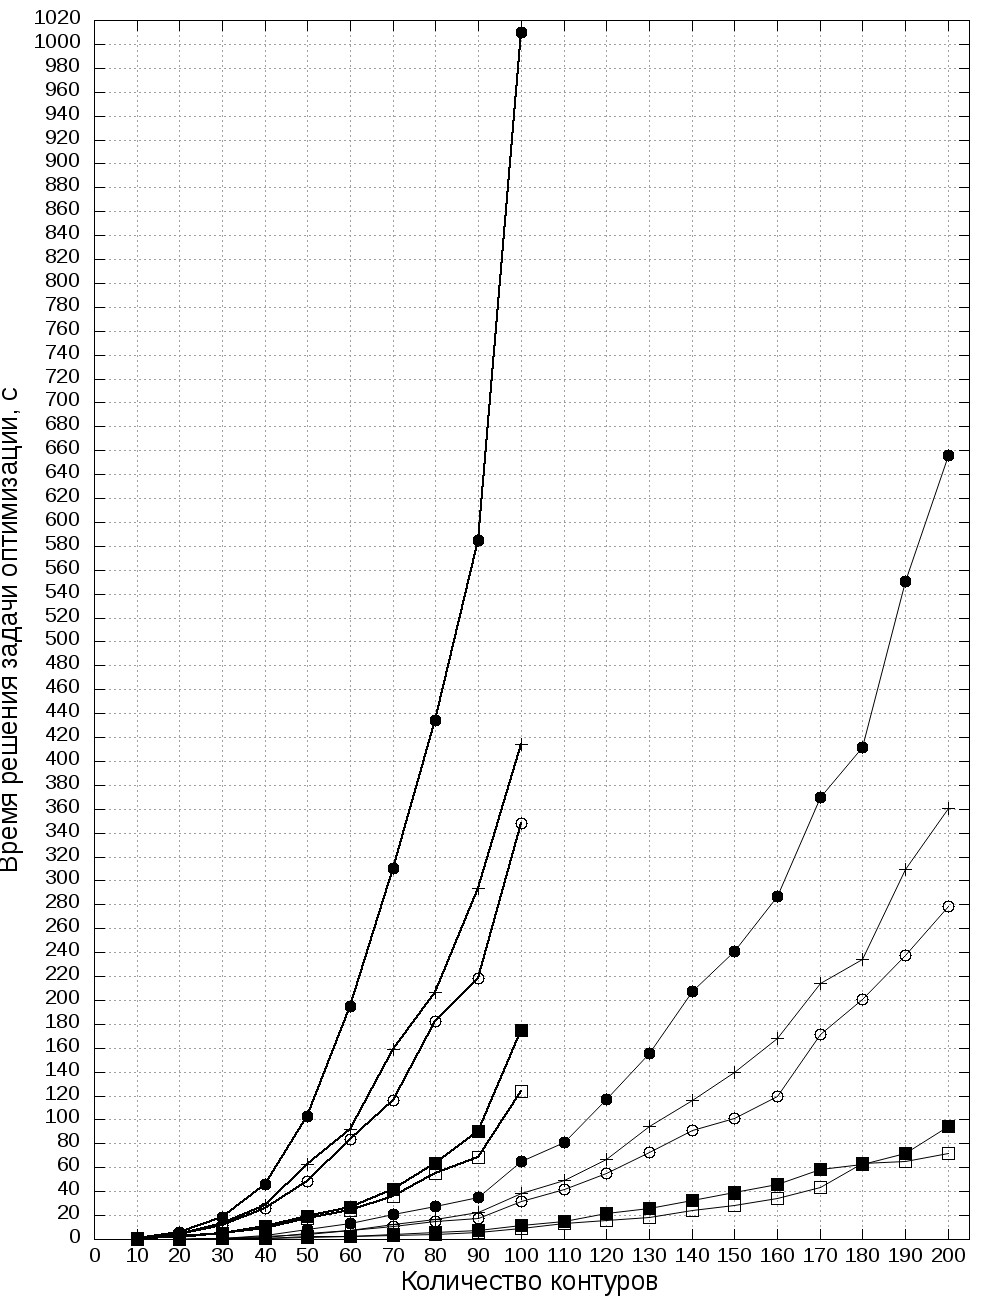
\includegraphics[width=\textwidth]{images/Problem-solution-time-graphs}
 \captionsetup{singlelinecheck=off}
 \caption{Время решения различных типов задач оптимизации на различных
 решателях:
 $\square$ -- $L_{\infty}$-задача на CPLEX,
 $\blacksquare$ -- $L_{1}$-задача на CPLEX,
 $\Circle$ -- $L_{\infty}$-задача на Ipopt,
 $\CIRCLE$ -- $L_{1}$-задача на Ipopt,
 $+$ -- $L_{2}$-задача на Ipopt. Для сравнения \textbf{жирными линиями} показаны
 графики времени решения задач оптимизации, из которых не были выброшены
 избыточные условия}
 \label{Problem-solution-time-graphs}
\end{figure}

На рисунке \ref{Problem-solution-time-graphs} изображены графики времени решения
задач оптимизации на различных решателях в различных метриках. Как оказалось,
задачи в $L_{1}$ и $L_{\infty}$ метриках решаются CPLEX примерно с одинаковой
скоростью, а на Ipopt -- задача в метрике $L_{1}$ решается даже медленнее, чем
в метрике $L_{2}$. Также на этом рисунке видно, каким образом предлагаемый
подход позволяет ускорить время работы алгоритма: он дает возможность за прежнее
время решить задачу в 2 раза большей размерности.

\textbf{8. Выводы и направления дальнейших исследований}. Из всего
вышесказанного можно сделать следующие выводы:

\begin{enumerate}
 \item Представленный метод позволяет отбросить в задаче восстановления
 выпуклого по измерениям его опорной функции значительную часть условий
 (около 80\% в рассмотренном примере).
 \item Благодаря этому можно значительно ускорить решение задачи оптимизации и
 увеличить допустимые размеры задачи, которые можно решить за разумное время
 \item Сам по себе алгоритм построения множества неизбыточных ограничений
 требует гораздо меньшего времени, чем задача оптимизации.
 \item Представленный метод восстановления тел с помощью решения задачи
 оптимизации, описанной выше, позволяет построить тело, наилучшим образом
 (с математической точки зрения) соответствующее к заданному набору теневых
 контуров.
 \item В полученном теле будет столько же граней, сколько сторон есть во всех
 теневых контурах вместе взятых. В этом заключается основной недостаток
 получаемых тел.
\end{enumerate}

Следующие направления представляются возможными для дальнейших исследований:

\begin{enumerate}
 \item В $L_{\infty}$-метрике представленную задачу можно решить и без
 решения задачи оптимизации: задача существования согласованного набора для
 заданного $\varepsilon$ решается за линейное время, поэтому с помощью деления
 отрезка пополам можно с любой заданной точностью найти такое минимальное
 $\varepsilon$, для которого существует согласованное решение.
 \item С точки зрения практики довольно ценно было бы рассмотреть задачу
 построения тела с заданным числом граней. Очевидно, что эту задачу можно
 сформулировать в виде задачи нелинейного программирования на линейном числе
 кусочно-линейных условий: условие того, что точка реализует максимум проекции
 на заданном направлении среди конечного набора точек может быть записано как
 неравенство между двумя (а не всеми) проекциями.
\end{enumerate}



\bibliographystyle{plain}
\bibliography{307167,81035,josaa-9-10-1693,234054,10.10022Fima.10007,906585citation,4586384,4333,141749,Gardner06convergenceof,Guntuboyina2012,cgal,how_to_cite_cgal,235821,glpk,clp,ipopt,ibm-ilog-cplex,WachterB06,hsl,openblas}

\end{document}